\documentclass[letterpaper,11pt,oneside,reqno]{article}

%%%%%%%%%%%%%%%%%%%%%%%%%%%%%%%%%%%%%%%%%%%%%%%%%%%%%%%%%%%%

\usepackage[pdftex,backref=page,colorlinks=true,linkcolor=blue,citecolor=red]{hyperref}
\usepackage[alphabetic,nobysame]{amsrefs}

%%%%%%%%%%%%%%%%%%%%%%%%%%%%%%%%%%%%%%%%%%%%%%%%%%%%%%%%%%%%
%main packages
\usepackage{amsmath,amssymb,amsthm,amsfonts,mathtools}
\usepackage{graphicx,color}
\usepackage{upgreek}
\usepackage[mathscr]{euscript}

%equations
\allowdisplaybreaks
\numberwithin{equation}{section}

%tikz
\usepackage{tikz}
\usetikzlibrary{shapes,arrows,positioning,decorations.markings}

%conveniences
\usepackage{array}
\usepackage{adjustbox}
\usepackage{cleveref}
\usepackage{enumerate}
\usepackage{datetime}
\usepackage{comment}

%paper geometry
\usepackage[DIV=12]{typearea}

%%%%%%%%%%%%%%%%%%%%%%%%%%%%%%%%%%%%%%%%%%%%%%%%%%%%%%%%%%%%
%draft-specific
\synctex=1
% \usepackage{refcheck,comment}

%%%%%%%%%%%%%%%%%%%%%%%%%%%%%%%%%%%%%%%%%%%%%%%%%%%%%%%%%%%%
%this paper specific
\newcommand{\ssp}{\hspace{1pt}}

%%%%%%%%%%%%%%%%%%%%%%%%%%%%%%%%%%%%%%%%%%%%%%%%%%%%%%%%%%%%
\newtheorem{proposition}{Proposition}[section]
\newtheorem{lemma}[proposition]{Lemma}
\newtheorem{corollary}[proposition]{Corollary}
\newtheorem{theorem}[proposition]{Theorem}
%%%%%%%%%%%%%%%%%%%%%%%%%%%%%%%%%%%%%%%%%%%%%%%%%%%%%%%%%%%%
\theoremstyle{definition}
\newtheorem{definition}[proposition]{Definition}
\newtheorem{remark}[proposition]{Remark}
%%%%%%%%%%%%%%%%%%%%%%%%%%%%%%%%%%%%%%%%%%%%%%%%%%%%%%%%%%%%

\newenvironment{lnotes}{\section*{Notes for the lecturer}}{}

\excludecomment{lnotes}

\begin{document}
\title{Lectures on Random Matrices
(Spring 2025) \\Lecture 2: Wigner semicircle law}


\date{Wednesday, January 15, 2025\footnote{\href{https://lpetrov.cc/rmt25/}{\texttt{Course webpage}}
$\bullet$ \href{https://lpetrov.cc/rmt25/rmt25-notes/rmt2025-l01.tex}{\texttt{TeX Source}}
$\bullet$
Updated at \currenttime, \today}}



\author{Leonid Petrov}


\maketitle



\begin{lnotes}
	PREP:
	\begin{enumerate}
		\item Start:
			Catalan number formula
		\item Moments of SC need to be computed
		\item
			SC is uniquely determined by its moments; need Carleman criterion to show that the moments determine the distribution.
		\item from expected moments to the full convergence, some analysis needed
	\end{enumerate}
\end{lnotes}


\section{Recap}

We are working on the Wigner semicircle law.
\begin{enumerate}
	\item Wigner matrices $W$:
		real symmetric random matrices with iid entries
		$X_{ij}$, $i>j$ (mean 0, variance $\sigma^2$);
		and iid diagonal entries $X_{ii}$ (mean 0, some other variance and distribution).
	\item Empirical spectral distribution (ESD)
		\begin{equation*}
			\nu_n = \frac{1}{n} \sum_{i=1}^{n} \delta_{\lambda_i/\sqrt{n}},
		\end{equation*}
		which is a random probability measure on $\mathbb{R}$.
	\item Semicircle distribution $\mu_{\mathrm{sc}}$:
		\begin{equation*}
			\mu_{\mathrm{sc}}(dx) = \frac{1}{2\pi} \sqrt{4-x^2} \, dx,
			\qquad x \in [-2,2].
		\end{equation*}
	\item Computation of expected traces of powers of $W$. We
		showed that
		\begin{equation*}
		\int_{\mathbb{R}} x^k \, \nu_n(dx) \to
			\#\left\{ \textnormal{rooted planar trees with $k/2$ edges} \right\}.
		\end{equation*}
\end{enumerate}

\section{Two computations}

First, we finish the combinatorial part,
and match the limiting expected traces of powers of $W$
to moments of the semicircle law.

\subsection{Moments of the semicircle law}

We also need to match the Catalan numbers to the moments of the semicircle law.
Let $k=2m$, and we need to compute
the integral
\begin{equation*}
	\int_{-2}^{2} x^{2m} \frac{1}{2\pi} \sqrt{4-x^2} \, dx.
\end{equation*}

By symmetry, we write:
\[
\int_{-2}^2 x^{2m}\rho(x)\, dx = \frac{2}{\pi} \int_0^2 x^{2m} \sqrt{4-x^2}\, dx.
\]

Using the substitution \(x = 2\sin\theta\), we have \(dx = 2\cos\theta\, d\theta\). The integral becomes:
\[
\frac{2}{\pi} \int_0^{\pi/2} (2\sin\theta)^{2m} (2\cos\theta) (2\cos\theta\, d\theta)
= \frac{2^{2m+2}}{\pi} \int_0^{\pi/2} \sin^{2m}\theta \cos^2\theta\, d\theta.
\]
Using \(\cos^2\theta = 1 - \sin^2\theta\), we split the integral:
\[
\frac{2^{2m+2}}{\pi} \left( \int_0^{\pi/2} \sin^{2m}\theta\, d\theta - \int_0^{\pi/2} \sin^{2m+2}\theta\, d\theta \right).
\]
Using the standard formula (cf. Problem \ref{prob:sin-integral})
\begin{equation}
	\label{eq:sin-integral}
\int_0^{\pi/2} \sin^{2n}\theta\, d\theta = \frac{\pi}{2} \frac{(2n)!}{2^{2n} (n!)^2},
\end{equation}
we compute each term:
\[
\frac{2^{2m+2}}{\pi} \left( \frac{\pi}{2} \frac{(2m)!}{2^{2m}(m!)^2} - \frac{\pi}{2} \frac{(2m+2)!}{2^{2m+2}((m+1)!)^2} \right).
\]
After simplification, this becomes
$C_m$, the $m$-th Catalan number.

\subsection{Counting trees and Catalan numbers}

Throughout this section, for a random matrix trace moment of order $k$,
we use $m=k/2$ as our main parameter. Note that $m$ can be arbitrary
(not necessarily even).

\begin{definition}[Dyck Path]
A \emph{Dyck path} of semilength $m$ is a sequence of $2m$ steps in the plane, each step being either $(1,1)$ (up step) or $(1,-1)$ (down step), starting at $(0,0)$ and ending at $(2m,0)$, such that the path never goes below the $x$-axis. We denote an up step by $U$ and a down step by $D$.
\end{definition}

\begin{definition}[Rooted Plane Tree]
A \emph{rooted plane tree} is a tree with a designated root vertex where the children of each vertex have a fixed left-to-right ordering. The size of such a tree is measured by its number of edges, which we denote by $m$.
\end{definition}

\begin{definition}[Catalan Numbers]
The sequence of \emph{Catalan numbers} $\{C_m\}_{m\geq 0}$ is defined recursively by:
\begin{equation}
	\label{eq:catalan-recurrence}
    C_0 = 1, \quad C_{m+1} = \sum_{j=0}^m C_j C_{m-j} \quad \text{for } m \geq 0.
\end{equation}
Alternatively, they have the closed form:
\begin{equation}
	\label{eq:catalan-closed}
    C_m = \frac{1}{m+1}\binom{2m}{m} =
		\binom{2m}{m} - \binom{2m}{m+1}.
\end{equation}
These numbers appear naturally in the moments of random matrices, where $m=k/2$ for trace moments of order $k$.
\end{definition}

\begin{lemma}
	\label{lemma:equivalence-catalan}
	Formulas
	\eqref{eq:catalan-recurrence} and \eqref{eq:catalan-closed} are equivalent.
\end{lemma}
\begin{proof}
	One can check that the closed form satisfies the recurrence relation by direct substitution. The other direction
	involves generating functions. Namely,
	\eqref{eq:catalan-recurrence} can be rewritten for the
	generating function
	\begin{equation*}
		C(z)=\sum_{m=0}^\infty C_m z^m
	\end{equation*}
	as
	\begin{equation*}
		C(z)=1+zC(z)^2.
	\end{equation*}
	Solving for $C(z)$, we get
	\begin{equation}
		\label{eq:catalan-generating}
		C(z)=\frac{1\pm \sqrt{1-4z}}{2z}.
	\end{equation}
	We need to pick the solution which is nonsingular at $z=0$,
	and it corresponds to the minus sign.
	Taylor expansion of the right-hand side of
	\eqref{eq:catalan-generating}
	at $z=0$
	gives the closed form.
\end{proof}

\begin{remark}
	\label{rmk:stanley-catalans}
	Catalan numbers enumerate many (too many!) combinatorial objects. For a comprehensive treatment, see \cite{stanley2015catalan}.
\end{remark}

\begin{proposition}[Dyck Path--Rooted Tree Correspondence]
	\label{prop:dyck-tree}
For any $m$, there exists a bijection between
the set of Dyck paths of semilength $m$ and the set of rooted plane trees with $m$ edges.
\end{proposition}

\begin{proof}
Given a Dyck path of semilength $m$, we build the corresponding rooted plane tree as follows
(see \Cref{fig:dyck_paths_m2} for an illustration):
\begin{enumerate}
    \item Start with a single root vertex
    \item Read the Dyck path from left to right:
        \begin{itemize}
            \item For each up step ($U$), add a new child to the current vertex
            \item For each down step ($D$), move back to the parent of the current vertex
        \end{itemize}
    \item The order of children is determined by the order of up steps
\end{enumerate}
This is clearly a bijection, and we are done.
\end{proof}


\begin{figure}[htpb]
\centering
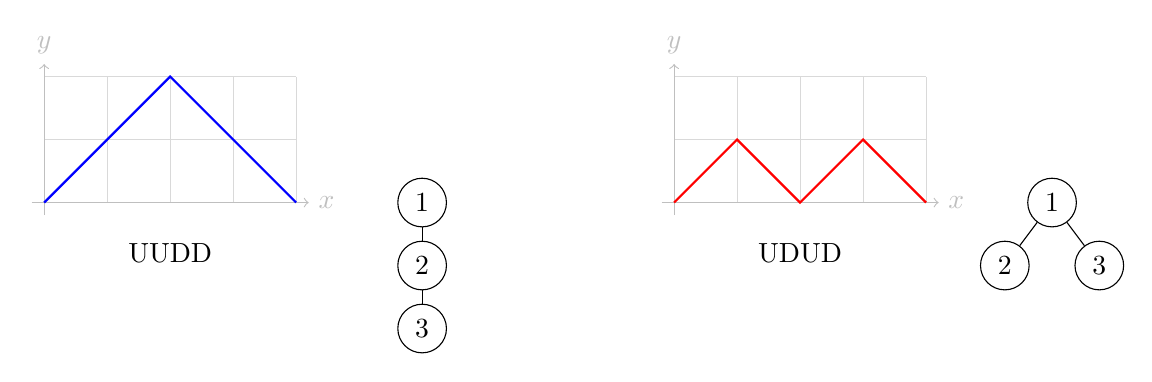
\begin{tikzpicture}[scale=0.8]
    % First Dyck path (UUDD)
    \begin{scope}[xshift=0cm]
        % Grid
        \draw[help lines,gray!30] (0,0) grid[step=1] (4,2);
        \draw[->,gray!50] (-0.2,0) -- (4.2,0) node[right] {$x$};
        \draw[->,gray!50] (0,-0.2) -- (0,2.2) node[above] {$y$};

        % Path
        \draw[thick,blue] (0,0) -- (1,1) -- (2,2) -- (3,1) -- (4,0);

        % Label
        \node[below] at (2,-0.5) {UUDD};
    \end{scope}

    % First tree
    \begin{scope}[xshift=6cm,level distance=1cm,
        every node/.style={circle,draw,minimum size=0.5cm}]
        \node (a) {1}
            child {node (b) {2}
                child {node (c) {3}}
            };
    \end{scope}

    % Second Dyck path (UDUD)
    \begin{scope}[xshift=10cm]
        % Grid
        \draw[help lines,gray!30] (0,0) grid[step=1] (4,2);
        \draw[->,gray!50] (-0.2,0) -- (4.2,0) node[right] {$x$};
        \draw[->,gray!50] (0,-0.2) -- (0,2.2) node[above] {$y$};

        % Path
        \draw[thick,red] (0,0) -- (1,1) -- (2,0) -- (3,1) -- (4,0);

        % Label
        \node[below] at (2,-0.5) {UDUD};
    \end{scope}

    % Second tree
    \begin{scope}[xshift=16cm,level distance=1cm,
        every node/.style={circle,draw,minimum size=0.5cm}]
        \node (a) {1}
            child {node (b) {2}}
            child {node (c) {3}};
    \end{scope}
\end{tikzpicture}
\caption{The two possible Dyck paths of semilength $m=2$ and their corresponding rooted plane trees.}
\label{fig:dyck_paths_m2}
\end{figure}

It remains to show that the Dyck paths or rooted plane trees are counted by the Catalan numbers, by verifying
the recursion \eqref{eq:catalan-recurrence} for them.
By \Cref{prop:dyck-tree}, it suffices to
consider only Dyck paths.

\begin{proposition}
	\label{prop:dyck-recurrence}
	The number of Dyck paths of semilength $m$ satisfies the Catalan recurrence \eqref{eq:catalan-recurrence}.
\end{proposition}
\begin{proof}
	We need to show that the number of Dyck paths of semilength $m+1$ is given by the sum in the right-hand side of \eqref{eq:catalan-recurrence}.
	Consider a Dyck path of semilength $m+1$,
	and let the \emph{first} time it
	returns to zero be at semilength $j+1$,
	where $j=0,\ldots,m$.
	Then the
	first and the $(2j+1)$-st steps are,
	respectively, $U$ and $D$.
	From $0$ to $2j+2$, the path does not return to the $x$-axis,
	so we can remove the first and the $(2j+1)$-st steps, and get a proper Dyck path of semilength $j$.
	The remainder of the Dyck path is a Dyck path of semilength $m-j$.
	This yields the desired recurrence.
\end{proof}
\begin{figure}[htbp]
	\centering
	\begin{tikzpicture}[scale=0.8]
		% Drawing the Dyck path with highlighted portions
		\draw[thick] (0,0) -- (1,1) -- (2,2) -- (3,1) -- (4,2) -- (5,1) -- (6,0)
		-- (7,1) -- (8,0)--++(1,1)--++(1,1)--++(1,-1)--++(1,-1)--++(1,1)--++(1,-1);

		% Axes and labels
		\draw[->] (-0.5,0) -- (16.5,0) node[right] {$x$};
		\draw[->] (0,-0.5) -- (0,4.5) node[above] {$y$};


		% Highlight important steps for recurrence explanation
		\draw[line width=2pt,red] (0,0) -- (1,1);
		\draw[line width=2pt,red] (5,1) -- (6,0);
	\end{tikzpicture}
	\caption{Illustration of a Dyck path decomposition for the proof of \Cref{prop:dyck-recurrence}.}
	\label{fig:dyck_recurrence}
\end{figure}


\section{Analysis steps in the proof}

We are done with combinatorics, and it remains to justify that
the computations lead to the desired semicircle law
from \href{https://lpetrov.cc/rmt25/rmt25-notes/rmt2025-l01.pdf}{Lecture 1}.

Let us remember that so far, we showed that
\begin{equation*}
	\lim_{n\to\infty}
	\frac{1}{n^{k/2+1}}
	\operatorname{\mathbb{E}}
	\left[
		\operatorname{Tr} W^k
	\right]
	=
	\begin{cases}
		\sigma^{2m} C_{m} & \text{if $k=2m$ is even}, \\
		0 & \text{if $k$ is odd}.
	\end{cases}
\end{equation*}
Here, $W$ is real Wigner
(unnormalized) with mean $0$,
where its off-diagonal entries are iid with variance $\sigma^2$.

\subsection{The semicircle distribution is determined by its moments}
\label{sub:carleman-semicircle}

We use (without proof)
the known Carleman's criterion for the uniqueness of a distribution by its moments.
\begin{proposition}[Carleman's criterion
	{\cite[Theorem~1.10]{shohat1943problem}}, \cite{Akhiezer1965Moment}]
	\label{prop:carleman}
	Let $X$ be a real-valued random variable with moments $m_k
	= \mathbb{E}[X^k]$ of all orders. If \[\sum_{k=1}^{\infty}
	(m_{2k})^{-1/(2k)} = \infty,\] then the distribution of
	$X$ is uniquely determined by its moments $(m_k)_{k\geq 1}$.
\end{proposition}
\begin{remark}
	By the Stone-Wierstrass theorem,
	the semicircle distribution is the unique distribution
	with compact support with these moments.
	However, we need to guarantee that there are no
	distributions on $\mathbb{R}$ with the same moments.
\end{remark}

Now, the moments satisfy the asymptotics
\begin{equation*}
	m_{2k}=C_k \sigma^{2k} \sim
	\frac{4^k}{k^{3/2}\sqrt{\pi}} \sigma^{2k},
\end{equation*}
so
\begin{equation*}
	\sum_{k=1}^{\infty} (m_{2k})^{-1/(2k)} \sim
	\sum_{k=1}^{\infty} \left( \frac{k^{3/2}\sqrt{\pi}}{4^k} \right)^{1/2k} \sigma^{-1}.
\end{equation*}
The $k$-th summands converges to $1/(2\sigma)$, so the
series diverges.

\begin{remark}
	See also Problem A.4 from \href{https://lpetrov.cc/rmt25/rmt25-notes/rmt2025-l01.pdf}{Lecture 1} on an example of a distribution not determined by its moments.
\end{remark}

\subsection{Convergence to the semicircle law}

Recall
\cite[Theorem~30.2]{billingsley1995probability}
that convergence
of random variables
in moments plus the fact that the
limiting distribution is uniquely determined by its moments
implies convergence in distribution.
However, we need weak in probability convergence,
which deals with random variables
\begin{equation*}
\int_{\mathbb{R}} f(x) \, \nu_n(dx),\qquad f\in C_b(\mathbb{R}),
\end{equation*}
and we did not compute the moments of these random variables.

To complete the argument, let us show that for each fixed integer \(k\ge1\),
we have almost sure convergence of the moments (of a
random distribution, so that the $Y_{n,k}$'s are random variables):
\[
Y_{n,k}\coloneqq\int_{\mathbb{R}}x^k\,\nu_n(dx)
  \;\xrightarrow[n\to\infty]{\text{a.s.}}\;
	m_{k},
	\qquad n\to\infty,
\]
where $m_k$ are the moments of the semicircle distribution,
and $\nu_n$ is the ESD corresponding to the scaling of the
eigenvalues as $\lambda_i/\sqrt n$.

As typical in asymptotic probability, we not only need the
expectation of $Y_{n,k}$, but also their variances,
to control the almost sure convergence.
Recall that
we showed $\operatorname{\mathbb{E}}(Y_{n,k})\to m_k$.
Let us assume the following:
\begin{proposition}[Variance bound]
	\label{prop:variance-bound}
	For each fixed integer \(k\ge1\) and large enough \(n\),
	we have
	\begin{equation*}
	\operatorname{\mathrm{Var}}(Y_{n,k})\le \frac{m_k}{n^2}.
	\end{equation*}
\end{proposition}
We will prove \Cref{prop:variance-bound} in \Cref{sub:variance-bound-proof}
below.
Let us finish the proof of convergence to the semicircle law modulo \Cref{prop:variance-bound}.


\subsubsection{A concentration bound and the Borel--Cantelli lemma}
From Chebyshev's inequality,
\[
  \mathbb{P}\Bigl(\bigl|Y_{n,k} - \mathbb{E}[Y_{n,k}]\bigr|
	\ge n^{-\frac{1}{4}}\Bigr)
  \le
  \operatorname{\mathrm{Var}}[Y_{n,k}]\sqrt{n}
	=O(n^{-\frac{3}{2}}),
\]
where in the last step we used \Cref{prop:variance-bound}.

Hence the probability that \(\lvert Y_{n,k} - \mathbb{E}[Y_{n,k}]\rvert > n^{-\frac{1}{4}}\) is summable in \(n\).  By the Borel--Cantelli lemma, with probability \(1\) only finitely many of these events occur.  Since \(\mathbb{E}[Y_{n,k}]\to m_k\), we conclude
\[
  \bigl|Y_{n,k} - m_k\bigr|
  \;\le\;\bigl|Y_{n,k}-\mathbb{E}[Y_{n,k}]\bigr|
  +\bigl|\mathbb{E}[Y_{n,k}]-m_k\bigr|
  \;\xrightarrow[n\to\infty]{}\;0
  \quad
  \text{almost surely.}
\]

\subsubsection{Tightness of \(\{\nu_n\}\) and subsequential limits}
\label{subsub:semicircle-tightness}

Since \(\lvert Y_{n,k}\rvert = \bigl|\int x^k\,\nu_n(dx)\bigr|\) stays
almost surely
bounded for each \(k\), one readily checks
(Problem \ref{prob:chebyshev-like})
that almost surely, for each fixed \(k\),
\begin{equation}
	\label{eq:chebyshev-like}
  \nu_n\bigl(\{x\,:\,|x|>M\}\bigr)
	\;\le\; \frac{C}{M^k}.
\end{equation}
By choosing \(k\) large, we see that \(\nu_n\) puts
arbitrarily little mass outside any large interval
\([-m,m]\).  Thus, the
sequence of probability measures
\(\{\nu_n\}\) is \emph{tight}.
By Prokhorov’s theorem \cite[Theorem~25.10]{billingsley1995probability},
there exists a subsequence \(\nu_{n_j}\) converging weakly to some probability measure \(\nu^*\).
We will now characterize all subsequential limits $\nu^*$ of $\nu_n$.

\subsubsection{Characterizing the limit measure}
\label{subsub:semicircle-characterization}

We claim that \(\nu^*=\mu_{\mathrm{sc}}\), the semicircle distribution
(and in particular, this measure is not random).
Indeed, fix \(k\).  Since \(x^k\) is a bounded function on a sufficiently large interval, and \(\nu_{n_j}\to\nu^*\) weakly, we have
\[
\int_{\mathbb{R}} x^k\,\nu_{n_j}(dx) \;\to\;\int_{\mathbb{R}} x^k\,\nu^*(dx).
\]
On the other hand, we have already shown
\[
\int_{\mathbb{R}} x^k \, \nu_{n_j}(dx)
   \;=\;
   Y_{n_j,k}
   \;\xrightarrow[j\to\infty]{\text{a.s.}}
   m_k
   \;=\;\int_{\mathbb{R}} x^k\,\mu_{\mathrm{sc}}(dx).
\]
Thus
\[
\int_{\mathbb{R}} x^k\,\nu^*(dx)
   \;=\;
   m_k
   \;=\;
   \int_{\mathbb{R}} x^k\,\mu_{\mathrm{sc}}(dx)
   \qquad
   \text{for all $k\ge1$.}
\]
By \Cref{prop:carleman}, the measure \(\nu^*\) is uniquely
determined by its moments.  Hence \(\nu^*\) must coincide
with \(\mu_{\mathrm{sc}}\).

\begin{remark}
	In \Cref{subsub:semicircle-tightness,subsub:semicircle-characterization}
	we tacitly assumed that we choose an elementary outcome $\omega$,
	and view $\nu_n$ as measures depending on $\omega$.
	Then, since the convergence of moments is almost sure,
	$\omega$ belongs to a set of full probability.
	The limiting measure $\nu^*$ must coincide
	with $\mu_{\mathrm{sc}}$ for this $\omega$,
	and thus, $\nu^*$ is almost surely nonrandom.
\end{remark}

Any subsequence of \(\{\nu_n\}\) has a further
sub-subsequence convergent to \(\nu\).  By a standard
diagonal argument, this forces \(\nu_n\to\nu\) in the weak
topology (almost surely).  This completes the proof that the ESD of our
Wigner matrix (rescaled by \(\sqrt{n}\)) converges to the
semicircle distribution weakly almost surely,
modulo \Cref{prop:variance-bound}.
(See also Problem \ref{prob:almost-sure-convergence}
for the weakly in probability convergence.)


\section{Proof of \Cref{prop:variance-bound}: bounding the variance}
\label{sub:variance-bound-proof}

There is one more ``combinatorial'' step in the proof of the
semicircle law: we need to show that the variance of the
moments of the ESD is bounded by \(m_k/n^2\).

Recall that
\[
	Y_{n,k}
	=\int_{\mathbb{R}}x^k\,\nu_n(dx)
	=\frac{1}{n^{1+\frac{k}{2}}}
	\sum_{i_1,\ldots,i_k=1}^{n} X_I,
	\quad
	\text{where}
	\quad
	X_I=X_{i_1 i_2}X_{i_2 i_3}\cdots X_{i_{k}i_1}.
\]
Here we use the notation $I$ for the multi-index $(i_1,\ldots,i_k)$,
and throughout the computation below,
we use the notation $I\in[n]^k$,
where $[n]=\{1,\ldots,n\}$.
We have
\[
\operatorname{\mathrm{Var}}\bigl(Y_{n,k}\bigr)
	=
	\frac{1}{n^{2+k}}
	\operatorname{\mathrm{Var}}
	\Bigl(\sum_{I\in[n]^k}X_I\Bigr)
	=
	\frac{1}{n^{2+k}}
	\sum_{I,J\in[n]^k}
	\operatorname{\mathrm{Cov}}\bigl(X_I,X_J\bigr).
\]
We claim that the sum of all covariances is bounded by a constant times~\(n^k\), which then implies
\(\operatorname{\mathrm{Var}}\bigl(Y_{n,k}\bigr)\le \mathrm{const}\cdot n^k / n^{2+k}=O\bigl(\tfrac{1}{n^2}\bigr)\).

\medskip

\noindent
\textbf{Step 1. Identifying when \(\operatorname{\mathrm{Cov}}\bigl(X_I,X_J\bigr)\) can be nonzero.}
For each \(k\)-tuple \(I=(i_1,i_2,\dots,i_k)\in[n]^k,\) the product
\[
	X_I = X_{i_1i_2}\,X_{i_2i_3}\,\dots \,X_{i_k i_1}
\]
is the product of the entries of our Wigner matrix corresponding to the directed ``edges''
\((i_1 \to i_2), (i_2 \to i_3),\dots,(i_k \to i_1)\).
Similarly, \(X_J\) is determined by the edges of another closed directed walk~\(J\).

\begin{enumerate}
\item
If \(I\) and \(J\) use disjoint collections of matrix entries, then \(X_I\) and \(X_J\) are independent, and hence $\operatorname{\mathrm{Cov}}(X_I,X_J)=0$.

\item
	If there is an edge (say, \(X_{i_1 i_2}\)) which appears
	\emph{only once}
	in exactly one of \(I\) or \(J\) but not both, then that
	edge factor is independent and forces
	$\operatorname{\mathrm{Cov}}(X_I,X_J)=0$ since
	$\operatorname{\mathbb{E}}[X_{i_1 i_2}]=0$.
Indeed, for example if \(X_{i_1 i_2}\) appears only in \(X_I\), then
\[
	\operatorname{\mathbb{E}}\left[ X_I \right]
	=
	\operatorname{\mathbb{E}}\left[ X_{i_1 i_2} \right]
	\cdot
	\operatorname{\mathbb{E}}\left[ \text{other factors} \right]
	=0,
	\qquad
	\mathbb{E}\bigl[X_I X_J\bigr]
	=
	\mathbb{E}[X_{i_1 i_2}]
	\cdot
	\mathbb{E}\bigl[\text{other factors}\bigr]
	=0.
\]

\end{enumerate}

\noindent
Thus, the only way we could get a nonzero covariance is if \emph{every} edge that appears in \(I\cup J\) appears at least twice overall.
Graphically, let us represent each \(k\)-tuple \(I\) by a directed closed walk in the complete graph on~\([n]\).  The union \(I\cup J\) must be a connected subgraph in which every directed edge has total multiplicity \(\ge2\).

\medskip

\noindent
\textbf{Step 2. Counting the contributions to the sum.}
Denote by \(q=\lvert V(I\cup J)\rvert\) the number of
distinct vertices involved in the union \(I\cup J\).
In principle, there are $O(n^q)$ ways to choose $q$ vertices from $[n]$.
Then we need to specify how the edges form two closed walks of length $k$.

We split into two cases:
\begin{enumerate}
\item
\(\boldsymbol{q\le k.}\)
Then the $n$-power in the sum over $I,J$ is at most
$n^k$, which yields the overall contribution
$O(n^{-2})$, as desired.

\item
\(\boldsymbol{q\ge k+1.}\)
Ignoring directions and multiplicities,
we see that the subgraph corresponding to $I\cup J$
contains at most \(k\) edges. Since \(q \ge k + 1\), we must have \(q = k + 1\)
(by connectedness). Thus,
\(I \cup J\) is a double tree.
Since $I$ and $J$ are subsets of this double tree and $q=k+1$,
they also must be double trees.
Thus, there exists an edge which appears in both $I$ and $J$, and
at least twice in $I$ and twice in $J$, so four times in $I\cup J$.
This contradicts the assumption that $I\cup J$ is a double tree.

This implies that
there are no leading contributions to the sum when \(q\ge k+1\).
\end{enumerate}

Combining these two cases, we conclude that the total number of pairs \((I,J)\) with nonzero covariance is of order at most \(n^k\),
This yields the desired bound on the variance, and completes the proof of \Cref{prop:variance-bound}.

With that, we are done with the Wigner semicircle law proof for real
Wigner matrices.  See Problem~\ref{prob:complex-wigner} for the complex case.

\section{Remark: Variants of the semicircle law}

Let us briefly outline a few examples
of the semicircle law for real/complex
Wigner matrices which relax the iid conditions and the
conditions that all moments of the entries must be finite.
This list is not comprehensive, it is presented as an illustration of the
universality / robustness of the semicircle law.
\begin{theorem}[Gaussian $\beta$-Ensembles \cite{Johansson_BGG_1998}, \cite{Forrester-LogGas}]
	Let $\beta > 0$, and consider an $n \times n$ random matrix ensemble with joint eigenvalue density:
\begin{equation}
	\label{eq:beta-density}
	p_n(\lambda_1,\ldots,\lambda_n) = \frac{1}{Z_{n,\beta}} \exp\left(-\frac{\beta}{4}\sum_{i=1}^n \lambda_i^2\right) \prod_{1\leq i<j\leq n} |\lambda_i-\lambda_j|^\beta
\end{equation}
where $Z_{n,\beta}$ is the normalization constant.\footnote{For
	$\beta=1,2,4$, this is the joint
eigenvalue density of the Gaussian Orthogonal, Unitary, and Symplectic Ensembles, respectively.
For general $\beta$, there is no invariant random matrix distribution
(while the eigenvalue density \eqref{eq:beta-density} makes sense), and
we can still treat all the $\beta$ cases in a unified manner.}
Then the ESD of the normalized eigenvalues $\lambda_i/\sqrt n$
converges weakly almost surely to the semicircle law.
\end{theorem}
\begin{theorem}[Correlated entries \cite{schenker2005semicircle}]
Let $W_n = \left(\frac{1}{\sqrt{n}} X_{pq}\right)_{1 \leq p,q \leq n}$
be a sequence of $n \times n$ Hermitian random matrices where:

\begin{enumerate}
\item The entries $X_{pq}$ are complex random variables that are:
		\begin{itemize}
		\item \textit{Centered:} $\operatorname{\mathbb{E}}[X_{pq}] = 0$,
		\item \textit{Unit variance:} $\operatorname{\mathbb{E}}[|X_{pq}|^2] = 1$,
		\item \textit{Moment bound:}
				$\displaystyle \sup_n \max_{p,q=1,\ldots,n} \operatorname{\mathbb{E}}\big[|X_{pq}|^k\big] < \infty$
				for all $k \in \mathbb{N}$.
		\end{itemize}

\item There exists an equivalence relation $\sim_n$ on pairs of indices $(p,q)$ in $\{1,\ldots,n\}^2$ such that:
		\begin{itemize}
		\item Entries $X_{p_1q_1},\ldots,X_{p_jq_j}$ are independent when
				$(p_1,q_1),\ldots,(p_j,q_j)$ belong to distinct equivalence classes.
		\item The relation satisfies the following bounds:
				\begin{enumerate}
			\item $\max_p \#\big\{(q,p',q') \in \{1,\ldots,n\}^3 \mid (p,q) \sim_n (p',q')\big\} = o(n^2)$,
				\item $\max_{p,q,p'} \#\big\{q' \in \{1,\ldots,n\} \mid (p,q) \sim_n (p',q')\big\} \leq B$ for some constant $B$,
				\item $\#\big\{(p,q,p') \in \{1,\ldots,n\}^3 \mid (p,q) \sim_n (q,p') \text{ and } p \neq p'\big\} = o(n^2)$.
				\end{enumerate}
		\end{itemize}

\item The matrices are Hermitian: $X_{pq} = \overline{X_{qp}}$.
	In particular, $(p,q)\sim_n (q,p)$, and this is consistent with the
	conditions on the equivalence relation.
\end{enumerate}

Then, as $n \to \infty$, the ESD of $W_n$ converges to the semicircle law.
\end{theorem}

There are variants of this theorem without the assumption
that all moments of the entries are finite.
\begin{theorem}[\cite{benaych-georges2016lectures}]
Let $M_n = [X_{ij}]_{i,j=1}^n$ be a symmetric $n \times n$ matrix with random entries such that:
\begin{itemize}
				\item The off-diagonal elements $X_{ij}$, for $i < j$, are i.i.d. random variables with $\operatorname{\mathbb{E}}[X_{ij}] = 0$ and $\operatorname{\mathbb{E}}[X_{ij}^2] = 1$.
				\item The diagonal elements $X_{ii}$ are i.i.d. random variables with $\operatorname{\mathbb{E}}[X_{ii}] = 0$ and a finite second moment, $\operatorname{\mathbb{E}}[X_{ii}^2] < \infty$, for $1 \leq i \leq n$.
\end{itemize}
Then the ESD of $M_n$, normalized by $\sqrt{n}$, converges to the semicircle law.
\end{theorem}

\begin{theorem}
For each $n \in \mathbb{Z}_+$, let $M_n = [X_{ij}]_{i,j=1}^n$ be a symmetric $n \times n$ matrix with random entries satisfying the following conditions:
\begin{itemize}
				\item The entries $X_{ij}$ are independent with $\operatorname{\mathbb{E}}[X_{ij}] = 0$ and $\operatorname{\mathbb{E}}[X_{ij}^2] = 1$.
				\item There exists a constant $C$ such that $\sup_{i,j,n} \operatorname{\mathbb{E}}\big[|X_{ij}|^4\big] < C$.
\end{itemize}
Then the ESD of $M_n$, normalized by $\sqrt{n}$, converges to the semicircle law almost surely. The second condition can also be replaced by a uniform integrability condition on the variances.
\end{theorem}

\begin{theorem}[For example, see \cite{silverstein1995empirical}]
Let $M_n = [X_{ij}]_{i,j=1}^n$ be a symmetric $n \times n$ matrix with random entries. Assume that the expected matrix $\operatorname{\mathbb{E}}[M_n]$ has rank $r(n)$, where
\[
\lim_{n \to \infty} \frac{r(n)}{n} = 0.
\]
Additionally, suppose $\operatorname{\mathbb{E}}[X_{ij}] = 0$, $\operatorname{\mathrm{Var}}(X_{ij}) = 1$, and
\[
\sup_{i,j,n} \operatorname{\mathbb{E}}\big[|X_{ij} - \operatorname{\mathbb{E}}[X_{ij}]|^4\big] < \infty.
\]
Then the ESD of $M_n$, normalized by $\sqrt{n}$, converges to the semicircle law almost surely.
\end{theorem}


\appendix
\setcounter{section}{1}

\section{Problems (due 2025-02-15)}

\subsection{Standard formula}
\label{prob:sin-integral}

Prove formula \eqref{eq:sin-integral}:
\begin{equation*}
	\int_0^{\pi/2} \sin^{2n}\theta\, d\theta = \frac{\pi}{2} \frac{(2n)!}{2^{2n} (n!)^2}.
\end{equation*}


\subsection{Tree profiles}
	Show that the expected height of a uniformly random Dyck path of semilength $m$ is of order~$\sqrt{m}$.

\subsection{Ballot problem}


Suppose candidate \(A\) receives \(p\) votes and candidate \(B\) receives \(q\) votes, where \(p > q \geq 0\). In how many ways can these votes be counted such that \(A\) is always strictly ahead of \(B\) in partial tallies?

\subsection{Bounding probability in the proof}
\label{prob:chebyshev-like}

Show inequality \eqref{eq:chebyshev-like}.

\subsection{Almost sure convergence and convergence in probability}
\label{prob:almost-sure-convergence}

Show that in Wigner's semicircle law,
the weakly almost sure convergence
of random measures $\nu_n$ to $\mu_{\mathrm{sc}}$
implies weak convergence in probability.

\subsection{Wigner's semicircle law for complex Wigner matrices}
\label{prob:complex-wigner}

Complex Wigner matrices are Hermitian symmetric, with iid complex off-diagonal
entries, and real iid diagonal entries (all mean zero).
Each complex random variable has independent real and imaginary parts.

\begin{enumerate}
	\item Compute the expected trace of powers of a complex Wigner matrix.
	\item Outline the remaining steps in the proof of
		Wigner's semicircle law for complex Wigner matrices.
\end{enumerate}



\bibliographystyle{alpha}
\bibliography{bib}


\medskip

\textsc{L. Petrov, University of Virginia, Department of Mathematics, 141 Cabell Drive, Kerchof Hall, P.O. Box 400137, Charlottesville, VA 22904, USA}

E-mail: \texttt{lenia.petrov@gmail.com}


\end{document}
